\documentclass{article}

\usepackage[final]{style}
\usepackage[utf8]{inputenc} % allow utf-8 input
\usepackage[T1]{fontenc}    % use 8-bit T1 fonts
\usepackage{hyperref}       % hyperlinks
\usepackage{url}            % simple URL typesetting
\usepackage{booktabs}       % professional-quality tables
\usepackage{amsfonts}       % blackboard math symbols
\usepackage{nicefrac}       % compact symbols for 1/2, etc.
\usepackage{microtype}      % microtypography
\usepackage{verbatim}
\usepackage{graphicx}       % for figures
\usepackage{caption}
\usepackage{hyperref}

%\title{Lecture 12: DIMENSIONALITY REDUCTION}

\title{Lecture 12: Face Recognition \& Dimensionality Reduction}

\author{
  \textbf{Kyu seo Ahn, Jason Lin, Mandy Lu, Liam Neath, Jintian Liang} \\
  Department of Computer Science\\
  Stanford University\\
  Stanford, CA 94305 \\
  \texttt{\{kyuseo, jason0, mlu355, lneath, jtliang\}@cs.stanford.edu} \\
}


\begin{document}

\maketitle

\section{Overview and Motivation}
\subsection{Overview}
Dimensionality reduction is a process for reducing the number of features to be used in an analysis or model. There are several methods commonly used in dimensionality reduction. The two main methods covered this lecture are Singular Value Decomposition (SVD) and Principal Component Analysis (PCA). 

\subsection{Motivation}
There are several reasons why reducing the dimensions for a model is useful.\\
\begin{enumerate}
\item Reduction in computational cost can be achieved. In many data sets, most of the variance can be explained by a relatively small number of principal components, when compared to the dimensionality of the entire feature set. By reducing our dimensions to focus on these key components, we can shrink the computational cost of analyzing each data point without losing much granularity in the data.

\item Reduce the effects of the “curse of dimensionality”. In lecture 11 we learned that as we increase the dimension of a feature space, the number of data points needed to “fill in” that space with the same density explodes exponentially. That is to say, the more dimensions there are, the more examples a machine learning algorithm needs to learn from and the longer the algorithm must run to analyze the same number of data points. By performing dimensionality reduction, we can mitigate the effects of this “curse of dimensionality”.

\item Compress data. By shrinking the dimensionality of an image, we can dramatically reduce the amount of storage required to store the image. 

In such cases the computational cost per data point may be reduced by many orders of magnitude with a procedure like SVD 
\end{enumerate}

\section{Singular Value Decomposition}
\subsection{Overview}
Intuitively, Singular Value Decomposition (SVD) is a procedure that allows one to (in a sense) "rotate the axes" of the feature space in which a dataset has been plotted so that instead of the different axes corresponding to specific features (e.g. age, income, gender, etc. of a customer) the new axes point in directions that track linear combinations of the original feature space.  These “new axes” are useful because they systematically break down the variance in the data points (how widely the data points are distributed) based on each directions contribution to the variance in the data:

% \begin{figure}[h!]
%   \caption{}
%   \centering
%   \includegraphics[width=0.5\textwidth]{Dimension_reduction_High_Level.png}
% \end{figure}
% * <kyuseoahn@gmail.com> 2017-11-07T22:40:47.042Z:
% 
% >   \includegraphics[width=0.5\textwidth]{Dimension_reduction_High_Level.png}
% cant get this image to load ahh
% 
% ^.

The result of this process is a ranked list of "directions" in the feature space ordered from most variance to least.  The directions along which there is greatest variance are referred to as the "principal components" (of variation in the data) and the common wisdom is that by focusing on the way the data is distributed along these dimensions exclusively, one can capture most of the information represented in in the original feature space without having to deal with such a high number of dimensions (but see below on the difference between feature selection and dimensionality reduction).

\subsection{Technical Details of Singular Value Decomposition}
\begin{itemize}
\item SVD represents any matrix	A as a product of three	matrices: $A = U\Sigma V^T$ where U and V are rotation matrices, and $\Sigma$ is a diagonal scaling matrix.	For example:\\
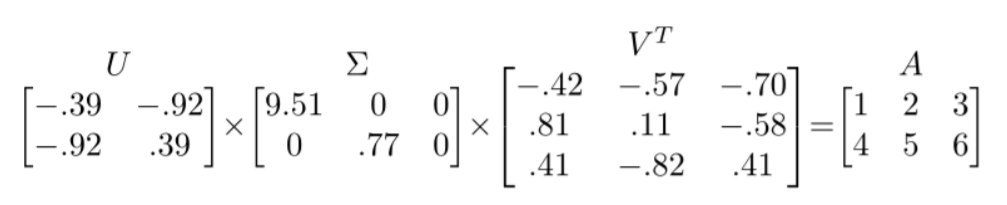
\includegraphics[scale = 0.5]{usigv_example}
\item For many readers, it may be sufficient to extract SVD values by writing: [U, S, V] = numpy.linalg.svd(A). However, the underpinnings of how SVD is computed is useful for later topics. Computers typically compute SVD by taking the following steps:
	\begin{itemize}
    	\item Compute the eigenvectors of $AA^{T}$. These vectors are the columns of U. Square root of the eigenvalues are the singular values (entries of $\Sigma$)
        \item Compute the eigenvectors of $A^{T}A$. These vectors are columns of V (or rows of $V^{T}$)
    \end{itemize}
\item Since SVD relies on eigenvector computation, which are typically fast, SVD can be performed quite quickly; even for large matrices.
\item A more detailed, geometric explanation of SVD may be found 
\href{http://www.ams.org/samplings/feature-column/fcarc-svd}{here}.
\end{itemize}

\subsection{Applications of Singular Value Decomposition}
\begin{itemize}
\item One the most utilized applications of SVD is the computation of matrix inverses. If an arbitrary matrix A can be decomposed by way of: $A = U\Sigma V^T$, the inverse of A may be defined as: $A^{+} = V^T \Sigma^{-1}U$. Although this inverse is an approximation, it allows one to calculate the inverses of many non-square matrices. MacAusland (2014) discusses the mathematical basis of this inverse, which is named the Moore-Penrose inverse, after its creators\cite{moore-penrose}. Unsurprisingly, a large variety of matrix problems can be solved be utilizing this approach. 
\item Singular Value Decomposition can also be used to compute the Principal Components of a matrix. Principal Components are heavily utilized in various data analysis and machine learning routines, hence SVD is typically a core routine within many programs.
\end{itemize}

\section{Principal Component Analysis}

\subsection{What are Principal Components?}
Continuing with the SVD example we have above, notice that Column 1 of U gets scaled by the first value from $\Sigma$.\\

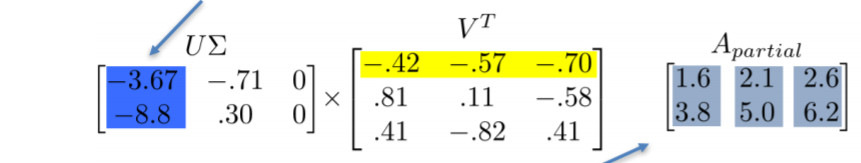
\includegraphics[scale = 0.5]{Usig}

Then, the resulting vector U$\Sigma$ gets scaled by row 1 of $V^T$ to produce a contribution to the columns of A which is denoted $A_{partial}$. Each product of (column i of U)*(value i from $\Sigma$)*(row i of $V^T$) produces a component of the final A.\\

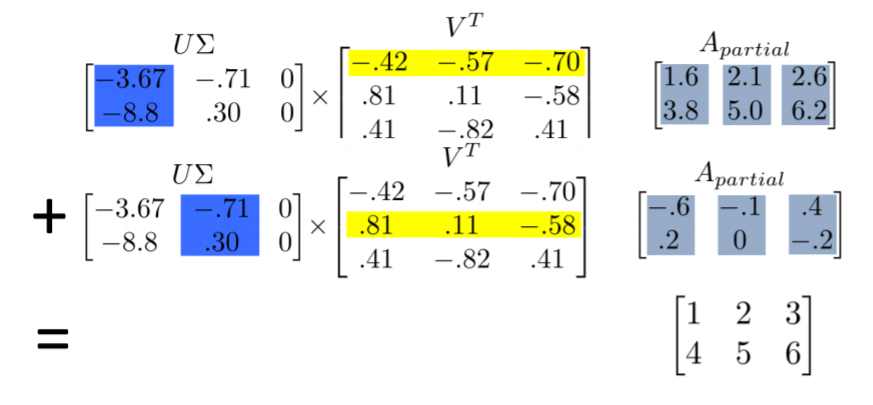
\includegraphics[scale = 0.5]{full_pca}

In this process we are building the the matrix A as a linear combination of the columns of U. As seen above, if we use all columns of U, we rebuild A perfectly. However, in real-world data, \textbf{we can use only the first few columns of U} to get a good approximation of A. This arises due to the properties that $\Sigma$ has. $\Sigma$ is a diagonal matrix where the largest value is in the top left corner, and the rest of the values on the diagonal decreases as you move to the right. Thus, the first few columns of $U$ contribute the largest weight towards $A$. These first few columns of U are called \textbf{principal components}.\\

However, not all matrices can be easily compressed as in the previous example. One way to figure out if it's worth performing is through Principal Component Analysis. From a high level standpoint, we want to see if there are certain 

\subsection{Performing Principal Component Analysis}
Principal Component Analysis can be performed using the sklearn package:
sklearn.decomposition.PCA. However, it was alluded to earlier that SVD can be used to perform Principal Component Analysis. A non-formal approach is outlined below:

\begin{enumerate}
\item Format your data into a $m * n$ matrix where $m$ denotes the number of samples and $p$ represents the number of features or variables corresponding to a single sample.
\item Center the matrix $X$ by subtracting the mean and dividing by the standard deviation along each column(feature) in $X$
\item Diagonalizing X using SVD yields: $X = U\Sigma V^{T}$
\item Eigenvectors are the principal directions and the projections on these axises are the components. This ultimately means we want to compute $XV$
\item Since V holds eigenvectors and is thus orthonormal, $XV = U\Sigma V^{T}V = US$
\item (5) implies we simply need the columns of $US$, both matrices that are surfaced by SVD
\end{enumerate}

Detailed explanations that elucidate the reasoning behind the above steps are discussed by Moore (1981) and can be found on numerous websites online.

\subsection{Applications of Principal Components}
\begin{itemize}
\item \begin{minipage}[t]{\linewidth}
	PCA has been extensively used in image compression. Much of the 	information captured within an image matrix can be extracted using matrices of lower ranks. This allows large images to be compressed without significant loss of quality. An example of PCA based compression, using only the first 16 principal components, is shown below:\\

  \centering
  
\includegraphics[width=\textwidth]{compare}
  \captionof{figure}{Right: Original Image, Left: Compressed Image}
  \label{fig:sample_figure}

\raggedright
$\,$\\
With just the first 16 principal components, an image that closely resembles the original image can be reconstructed. The relative error as a result of the dimensions used for PCA for the above image is shown below:

  \centering
  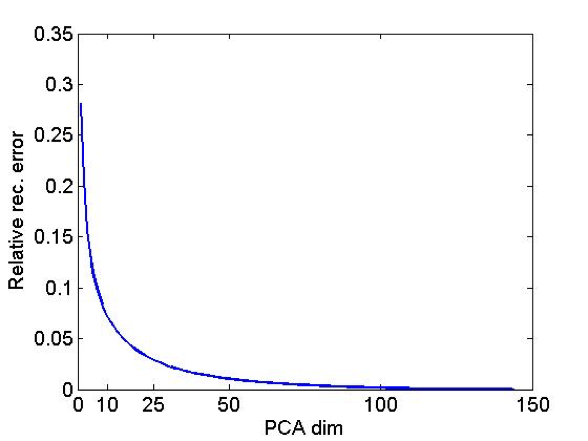
\includegraphics[width=\textwidth]{PCA_dim}
  \captionof{figure}{Relative Error as Function of PCA dimensions}
  \label{fig:sample_figure}
\end{minipage}

\item Web search engines also utilize PCA. There are billions of pages on the Internet that may have a non-trivial relation to a provided search phrase. Companies such as Google, Bing and Yahoo typically narrow the search space by only considering a small subset of this search matrix, which can be extracted using PCA (Abdulla \& Snasel, 2009). This is critical for timely, efficient searches and speaks to the power of SVD.
\end{itemize}

In essence, PCA allows you to represent data samples as weights on various components - allowing one to essentially represent the difference between samples. This can significantly reduce data redundancy and can make algorithms used in a variety of industries more efficient and insightful!

% References
\small
\bibliographystyle{plain}
\bibliography{bibliography}

% \section{References}
% \begin{enumerate}
% \item MacAusland, R. (2014). The Moore-Penrose Inverse and Least Squares. Tacoma, Washington: University of Puget Sound.
% \item Abdulla H.D., Snasel V. (2009) Search Result Clustering using a Singular Value Decomposition (SVD) Proceedings of the First International Conference on Intelligent Human Computer Interaction. Springer, New Delhi
% \end{enumerate}

% Given a model with very high variance, how do you reduce variance
% - variance is high when model complexity is high
% - for example, increase the k for k-nearest neighbors to smooth out decision boundaries, thus simplifying model
% - regularize your parameters
% - get more training data to get more representation from the world

% You should know your data (how much supervision, how noisy, how much you’re willing to pay for training data)
% Know your goals
% Basically, understand your model and what the algorithms and parameters mean

% Give image features and training labels to algorithm to get a classifier
% Run classifier on new images to get a prediction

% Image Features
% 1. Color
%     1. Invariant w.r.t. translation or rotation
%     2. Varying w.r.t. occlusion (hiding part of the image)
%     3. Scaling is more complicated, since blowing things up might increase some colors
% 2. Global Shape (PCA Space)
%     1. invariant w.r.t. translation, rotation
%     2. complicated with scale
% 3. Local shape (shape context)
%     1. invariant w.r.t. translation, scale
%     2. complicated with rotation
% 4. Texture
%     1. invariant w.r.t translation

% Singular Value Decomposition (SVD)
% - “factorize” a matrix, representing it as the product of some other matrices
% - total image size decreases, since M = N X O

% 2X2, 2X2, 2X2
% U(Sigma)V^{T} = A
% - sigma as diagonal matrix with largest value in the top left corner
% No gains here, but gains will come from larger matrix dimensions
% U and V are rotation matrices
% Sigma is a diagonal matrix
% Column 1 of U gets scaled by the first value from Sigma
% So the first column of U(Sigma) and first row in V^{T} gives the most information because the top-left value of Sigma is the largest
% Building A as linear combination of the columns of U
% The first few columns of U are the Principal Components of the data

% If A is symmetric, then you can break it down to Phi Sigma Phi^{T}

% Suppose given square matrix A. Can solve for vector x and scalar lambda s.t. A x = lambda x
% Finding eigenvectors:
% x = some random unit vector
% while(x hasn’t converged): 
% 	x = Ax
% 	normalize x
% Eigenvectors are for square matrices, but SVD is for all matrices
% Take eigenvectors of AA^{T} (matrix is always square)
% 	1. These eigenvectors are the columns of U
% 	2. Square root of eigenvalues are the singular values (entries of Sigma)
% Take eigenvectors of A^{T}A (matrix is always square)
% 	1. These eigenvectors are columns of V (or rows of V^{T})
% SVD is fast, even for large matrices

% SVD just shows that this can be done. Principal Component Analysis (PCA) is how decomposition is done

% PCA
% covariance as a measure of how much each of the dimensions vary from the mean with respect to each other
% covariance(X,Y) = \sum\limits_{i=1}^{n}\frac{(X_{i}-X_{bar})((Y_{i}-Y_{bar})}{n - 1}
% What is the interpretation of covariance?
% - No good interpretation. The only good interpretation is from their sign
% - positive meaning positive correlation, same with negative
% - Covariance of 0 means that the two dimensions are independent of each other
% Trying to maximize covariance
% 1. Project set of 2D data points x onto a 1D line
% X is a Gaussian that has some mean vector (same dimensions as X), covariance matrix Sigma
% Since Gaussians are symmetric, its covariance is also symmetric.
% Sigma = U Delta^{1/2}(U Delta^{1/2})^{T}
% Can represent original data as X ~ mu + U N(0, Delta)
% Principal components of Sigma are the eigenvectors
% Principal lengths of Sigma are the eigenvalues
% - Not flat if sigma_{1} \approx sigma_{2} -> don’t compress data
% - flat if sigma_{1} >> sigma_{2} -> can represent as fewer dimensions so compress
% PCA Algorithm
% 	1. Find mean along dimension
% 	2. Find covariance matrix
% 	3. Compute eigenvalues and eigenvectors of covariance matrix
% 	4. Order eigenvalues
% Given new image
% 1. Subtract mean from each point to get t’
% 2. Project onto eigenvector space where y=At’, where A is the principal components that you keep
% 3. use T’ = {y_{1}…y_{n}} to test

% PCA by SVD
% 1. Take all data points to get A, find SVD decomposition M Pi N^{T} where M is a column orthonormal matrix of left singular vectors and N_{T} is a row orthonormal matrix
%     1. MM^{T} = NN^{T} = I
% 2. Compute sample mean
% 3. Center the data by subtracting the mean from each column of X to get X_{c}
% 4. Get sample covariance matrix
% 5. Do SVD of Sigma to get 1/n N Pi^{2} N^{T}
%     1. N is orthonormal and Pi is diagonal 

% Image Compression
% Take patches (nxn) pixels on a grid, view each as n^{2} dimensional vector
% Perform PCA
\end{document}
